\documentclass[11pt, a4paper]{article}
\usepackage[utf8]{inputenc}
\usepackage[spanish]{babel}
\usepackage{graphicx}   
\usepackage{float}   
\usepackage{fontspec}
\usepackage{setspace}
\usepackage{anyfontsize}
\usepackage{hyperref}
\usepackage[style=apa7, backend=biber]{biblatex}
\addbibresource{referencias.bib}
\DeclareLanguageMapping{spanish}{spanish-apa}
\hypersetup{
    colorlinks=true,
    linkcolor=black,
    citecolor=magenta,
    urlcolor=cyan,
    pdftitle={Musy Documentación},
    pdfauthor={Beltrán González Martos}
}
\usepackage{listings}
\usepackage{xcolor-material}
\definecolor{codebackground}{rgb}{0.95,0.95,0.95}
\lstset{
    backgroundcolor=\color{codebackground},
    basicstyle=\ttfamily\footnotesize,
    breaklines=true,
    frame=single,
    numbers=left,
    numberstyle=\tiny\color{gray}
}
\onehalfspacing
\setmainfont{IBM Plex Serif}

\begin{document}

\begin{titlepage}
    \centering

    
\includegraphics[width=0.4\textwidth]{media/logo-litterator.png}

    \fontsize{26pt}{24pt}\selectfont \textbf{Trabajo Fin de Grado} \\
    \vspace{4.5cm}
    
    \fontsize{24pt}{24pt}\selectfont \textbf{Musy} \\
    \vspace{0.5cm}
    
\includegraphics[width=0.2\textwidth]{media/Square310x310Logo.png} \\
    \vspace{2cm}

    \hfill
    \begin{minipage}{0.8\textwidth}
        \raggedleft
        \large
        \begin{spacing}{1.5}
            \textbf{Autor:} Beltrán González Martos \\
            \textbf{Tutor:} Héctor Ángeles Borrás \\
            Desarrollo de Aplicaciones Multiplataforma \\
            \textbf{Fecha:} 9 de junio de 2025
        \end{spacing}
    \end{minipage}

    


\end{titlepage}

\pagenumbering{gobble}

\begin{abstract}
    Este proyecto aborda la ausencia de reproductores de musica offline modernos además de abordar el alto consumo de recursos en aplicaciones web, proponiendo una solución basada en tauri (Rust + Angular) para garantizar eficiencia. Se desarrolló una aplicación de escritorio compatible con Linux, MacOs y Windows, priorizando la optimización de memoria y la experiencia de usuario. El resultado es una aplicación escalable con arquitectura modular para futuras extensiones, validando así el potencial de Tauri en aplicaciones de escritorio.
\end{abstract}

\noindent \textbf{Palabras clave}: Tauri, Rust, Angular, reproductor de música, rendimiento, UI moderna.

\selectlanguage{english}
\begin{abstract}
    This project addresses both the lack of modern offline music players and the high resource consumption in web applications by proposing an efficient solution based on Tauri (Rust + Angular). A cross-platform desktop application was developed for Linux, MacOs, and Windows, with the particular emphasis on memory optimization and user experience. The result is a scalable application with modular architecture for future extensions, demonstrating Tauri's potential for desktop applications.
\end{abstract}

\noindent \textbf{Keywords}: Tauri, Rust, Angular, music player, performance, modern UI.

\selectlanguage{spanish}

\clearpage

\tableofcontents
\listoffigures
\listoftables
\lstlistoflistings


\clearpage


\pagenumbering{arabic}
\setcounter{page}{1}
\section{Introducción}

Con el aumento de precios y la inclusión de anuncios en las suscripciones premium de plataformas multimedia como Spotify o iTunes, se prevé un resurgimiento de la reproducción local de música. Este proyecto tiene como objetivo ofrecer una alternativa moderna, intuitiva y sencilla frente a las aplicaciones de reproducción local existentes.


\section{Justificación del tema elegido}

Aunque existen alternativas a las aplicaciones de reproducción en streaming, resulta difícil encontrar una que combine una interfaz moderna, atención al detalle y código abierto (open-source). Por ello, se ha desarrollado esta propuesta, centrada en una aplicación de reproducción local con una interfaz similar a Spotify o iTunes, lo que facilitará la transición de nuevos usuarios.

\section{Objetivos}

El objetivo principal es desarrollar una aplicación multiplataforma basada en tecnologías web, eficiente en la gestión de recursos del sistema y fácil de usar. Adicionalmente, se busca que el proyecto sirva como aprendizaje en el uso de Angular y Rust.

\section{Metodología}

Para la realización del proyecto se empleará la metodología ágil SCRUM. En este caso, el autor asumirá los roles de product owner, scrum master y development team. Las tareas serán asignadas diariamente, y se realizará un seguimiento continuo del progreso.

\section{Tecnologías y herramientas usadas en el proyecto}

Este proyecto está desarrollado mediante un conjunto de tecnologías modernas
distribuidas en tres capas principales:

    \begin{itemize}
        \item \textbf{Frontend}: Angular 17, Tailwind CSS V4
        \item \textbf{Backend}: Rust, Tauri 2.0
        \item \textbf{Base de Datos}: SQLite
    \end{itemize}

    \subsection{Razones}

    La selección de tecnologías para este proyecto se ha basado en los siguientes criterios técnicos y de eficiencia: 

        \begin{itemize}
            \item \textbf{Angular 17}: Se ha elegido este framework por su arquitectura basada en componentes, que favorece la escalabilidad y mantenibilidad del código. Además, se ha considerado relevante la oportunidad de explorar alternativas a React, ampliando así el conocimiento en ecosistemas frontend modernos.
            \item \textbf{Tailwind CSS v4}: Se ha optado por esta herramienta debido a su eficiencia en el desarrollo de interfaces responsive, así como a la familiaridad previa con su paradigma utility-first, lo que permite agilizar el proceso de diseño.
            \item \textbf{Rust}: Se ha seleccionado este lenguaje por su rendimiento optimizado y seguridad. Además, representa una valiosa oportunidad de aprendizaje de un lenguaje de programación de bajo nivel.
            \item \textbf{Tauri}: Se ha preferido sobre alternativas como Electron debido a su menor consumo de recursos y mejor rendimiento en aplicaciones de escritorio multiplataforma.
            \item \textbf{SQLite}: Se ha implementado este sistema de gestión de bases de datos por su ligereza, y adecuación a los requisitos del proyecto.
        \end{itemize}

    El entorno de desarrollo está configurado en Visual Studio Code, utilizando extensiones específicas para cada tecnología mencionada, lo que garantiza un flujo de trabajo eficiente.

\section{Especificación de Requisitos de Software}



\section{Despliegue y pruebas}

En este apartado se detallan los pasos seguidos para el despliegue de la aplicación de escritorio, así como las pruebas realizadas para garantizar su correcto funcionamiento.

        \subsection{Despliegue de la aplicación}

        Se elaboró un proceso de empaquetado y distribución de la aplicación utilizando Tauri, que permite generar ejecutables multiplataforma (Windows, MacOs, Linux). Para ello:

        \begin{itemize}
            \item Se utilizó el sistema de bundling de Tauri para empaquetar los recursos frontend (Angular) junto al backend (Rust).
            \item Se generaron instaladores específicos para diferentes sistemas operativos: \begin{itemize}
                \item \textbf{.AppImage} para Linux
                \item \textbf{.exe} para Windows
                \item \textbf{.dmg} para MacOs
                \end{itemize}
        \end{itemize}

        \subsection{Pruebas realizadas}

        Con el objetivo de validar la funcionalidad y estabilidad de la aplicación, se llevaron a cabo las siguientes pruebas:

            \subsubsection{Pruebas de integración}

            \begin{itemize}
                \item Se comprobó la comunicación entre el frontend y el backend, asegurando que las llamadas desde Angular a Rust (a través de Tauri) funcionaban correctamente.
                \item Se testearon casos como la carga de archivos de audio, reproducción en diferentes formatos y manejo de errores.
            \end{itemize}

            \subsubsection{Pruebas de usabilidad}

            \begin{itemize}
                \item Se realizaron test con usuarios reales para evaluar la experiencia de uso (UX), recogiendo feedback sobre la interfaz y la fluidez de la reproducción musical.
                \item Se analizaron posibles cuellos de botella en el rendimiento, especialmente al manejar playlist con muchas canciones o archivos de alta resolución.
            \end{itemize}

        La aplicación fue testeada en los tres sistemas operativos principales (Windows, MacOs y Linux), aunque el desarrollo se centró principalmente en las versiones para MacOs y Linux. \\

        El rendimiento de la aplicación resulta significativamente mejorado al aprovechar las características nativas de Tauri, en comparación con soluciones basadas en Electron. \\

        \begin{figure}[h!]
            \centering
            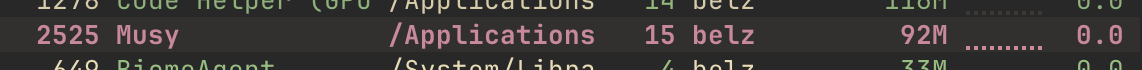
\includegraphics[width=0.8\textwidth]{media/imagemusyram.png}
            \caption{Rendimiento de la aplicación en MacOs}
            \label{fig:ejemplo}
        \end{figure}

\section{Estado del arte}

En la actualidad, el panorama de reproducción musical se divide principalmente en dos enfoques: plataformas de streaming y reproductores locales tradicionales. A continuación, se analizan sus características, ventajas y desventajas.

        \subsection{Plataformas de streaming}

        Las plataformas de streaming (Spotify, Apple Music, etc...) dominan el mercado actual debido a:

        \begin{itemize}
            \item Acceso instantáneo a catálogos musicales extensos (más de 100 millones de canciones).
            \item Interfaces modernas con recomendaciones basadas en algoritmos.
            \item Sincronización multiplataforma (dispositivos móviles, web y escritorio).
        \end{itemize}

        Sin embargo, presentan limitaciones significativas:

        \begin{itemize}
            \item Dependencia de conexión a internet permanente.
            \item Modelo de negiocio basado en suscripciones o publicidad invasiva.
            \item Falta de propiedad real sobre la música (acceso condicionado al pago).
        \end{itemize}

        \subsection{Reproductores locales tradicionales}

        Los reproductores de música offline (Winamp, Strawberry, etc...) ofrecen:

        \begin{itemize}
            \item Control completo sobre los archivos musicales (propiedad permanente).
            \item Uso sin restricciones de conectividad o cuentas de usuario.
            \item Menor consumo de recursos al evitar dependencias en la nube.
        \end{itemize}

        No obstante, adolecen de problemas críticos:

        \begin{itemize}
            \item Interfaces obsoletas y experiencias de usuario poco intuitivas.
            \item Dificultad para encontrar versiones actualizadas (muchos proyectos estan abandonados).
            \item Limitada compatibilidad con formatos modernos o sistemas operativos recientes.
        \end{itemize}

        \subsection{Mi propuesta}

        Este análisis evidencia la necesidad de reproductores locales que combinen:

        \begin{itemize}
            \item Diseño contemporáneo (similar al streaming).
            \item Independencia de infraestructuras en la nube.
            \item Soporten estándares actuales (formatos lossless, metadatos avanzados).
        \end{itemize}

        La solución propuesta en este proyecto busca ocupar este espacio, aprovechando tecnologías modernas (Tauri, Rust, Angular) para superar las limitaciones de ambas aproximaciones.

\section{Profundización de conceptos}

En esta sección se explicarán en detalle los componentes principales de la aplicación.

        \subsection{Frontend}

        Angular

            \subsubsection{Playbar}

            \begin{figure}[H]
                \centering
                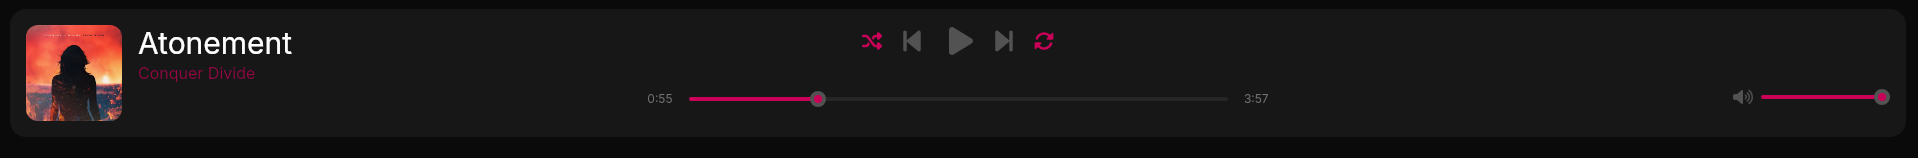
\includegraphics[width=1\textwidth]{media/screenshots/playbar.png}
                \caption{Playbar}
                \label{fig:playbar}
            \end{figure}

            El componente principal para la reproducción de música está compuesto por tres contenedores \verb|div|:

            \begin{itemize}
                \item \textbf{Izquierdo}. En el primero se muestran la portada de la canción, el título y el artista.
                \item \textbf{Central}. El segundo contiene dos subcontenedores: uno para los botones de control (reproducción, aleatorio, anterior/siguiente, repetición) y otro para la barra de progreso.
                \item \textbf{Derecho}. El tercero incluye exclusivamente la barra de volumen. En futuras iteraciones podría implementarse un botón para gestionar la cola de reproducción.
            \end{itemize}

            La parte del componente de typescript contiene únicamente métododos que llaman al servicio de manejo de canciones \verb|song-management.service.ts|.

            \subsubsection{Sidebar}

            \begin{figure}[H]
                \centering
                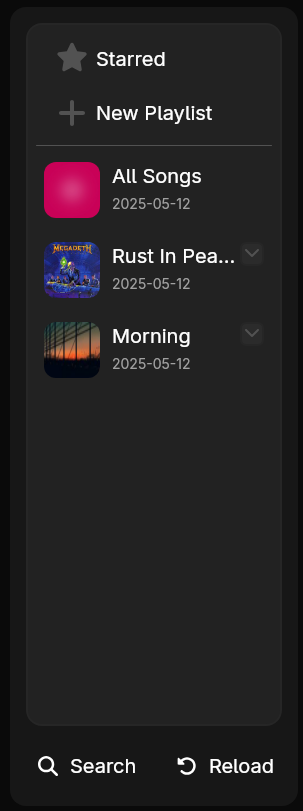
\includegraphics[width=0.4\textwidth]{media/screenshots/sidebar.png}
                \caption{Sidebar}
                \label{fig:sidebar}
            \end{figure}

            Componente donde se interactua con las playlist, ya sea creando nuevas o borrando las existentes. Contiene diversos botones para navegar por la aplicación.

            Estos son sus atributos:

            \begin{lstlisting}[caption={Atributos Y Constructora Sidebar}]
playlists: Playlist[] = []
name:string = ""
isModalOpen:boolean = false;
isModalOpenSearch:boolean = false;
songs:Song[] = []
filteredSongs:Song[] = []
coverPath: string = "assets/black.jpg"

constructor (public mainScreenStatus:MainScreenStatusService, public songManagement:SongManagementService) {}
            \end{lstlisting}

            Serán explicados más adelante.

                \paragraph{Playlist}
                ‎ 

                El componente gestiona la representación y comportamiento de las listas de reproducción en la interfaz. Su estructura básica comprende:

                \begin{lstlisting}[caption={Atributos y Constructora Playlist}]
coverPath = 'assets/black.jpg';

isDropDownOpen: boolean = false;

constructor (public mainScreenStatus:MainScreenStatusService) {}

@Input() playlistId!: number;

@Input() playlistName!: string;

@Input() playlistDate!: string;

@Input() playlistCoverPath!: string;

@Input() playlistIsStarred!: boolean;

@Input() refreshFn!: () => void;
                \end{lstlisting}

                Cada instancia de \verb|Playlist| actúa como elemento interactivo que actualiza el componente \verb|mainscreen| mediante un servicio. Utiliza el patrón de decoradores \verb|@Input| para recibir propiedades del componente padre. Gestiona un menú desplegable mediante el atributo \verb|isDropDownOpen|.
                
                Algunos de los métodos más importantes de este componente destacan:

                \begin{lstlisting}[caption={getCoverPath()}]

async getCoverPath(): Promise<string> {
    if (!this.coverPath) return 'assets/black.jpg';
    console.log("Hola")

    const fileData = await readFile(this.playlistCoverPath);
        
    const blob = new Blob([fileData], { type: 'image/jpeg' });

    if (this.coverPath) {
        URL.revokeObjectURL(this.coverPath);
    }

    return URL.createObjectURL(blob);
}
                \end{lstlisting}

                Este método se encarga de:
                \begin{enumerate}
                    \item Verificar la existencia de una ruta de portada válida.
                    \item Convertir la imagen local en un objeto \verb|Blob| mediante:
                    \begin{itemize}
                        \item Lectura del archivo con \verb|readFile|
                        \item Creación de URL temporal con \verb|URL.createObjectURL|
                    \end{itemize}
                    \item Liberar recursos previos con \verb|URL.revokeObjectURL|
                    \item Proporcionar fallback a imagen predeterminada (\verb|black.jpg|)
                \end{enumerate}

                \begin{lstlisting}[caption={Dropdown}]
toggleDropDown() {
    this.isDropDownOpen = !this.isDropDownOpen;
  }

  closeDropDown() {
    this.isDropDownOpen = false;
  }

  @HostListener('document:click', ['$event'])
  onClickOutside(event: Event) {
    const target = event.target as HTMLElement;
    if (!target.closest('.relative.inline-block')) {
      this.closeDropDown();
    }
  }
                \end{lstlisting}

                Por motivos de diseño, se ha implementado un menú desplegable (dropdown) que contiene acciones específicas para cada playlist. El estado de visualización se controla mediante la variable \verb|isDropDownOpen|, que se alterna con \verb|toggleDropDown()|. El cierre automático se gestiona mediante un \verb|@HostListener| que detecta clics fuera del área del componente. Actualmente, el menú incluye la opción de eliminación de playlists, pero su diseño permite la incorporación de nuevas funcionalidades como marcado como favorito o edición avanzada en futuras iteraciones.

                \begin{figure}[H]
                    \centering
                    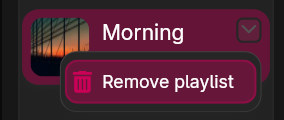
\includegraphics[width=0.6\textwidth]{media/screenshots/remove_playlist.png}
                    \caption{Eliminar playlist}
                    \label{fig:eliminar playlist}
                \end{figure}

                \begin{lstlisting}[caption={removePlaylist()}]
async removePlaylist() {
    const data_dir = await appDataDir();
    invoke('remove_playlist', {playlist_id: this.playlistId, db_path: data_dir});
    this.refreshFn();
  }
                \end{lstlisting}

                El método \verb|removePlaylist()| se encarga de gestionar la eliminación de playlists mediante un proceso que consta de tres etapas principales: primero, se obtiene el directorio de datos de la aplicación mediante \verb|appDataDir()|; a continuación, se realiza una llamada al backend mediante \verb|invoke()|, enviando como parámetros el identificador de la playlist (\verb|playlist_id|) y la ruta de la base de datos (\verb|db_path|); finalmente, se ejecuta la función \verb|refreshFn()| para actualizar la interfaz. La implementación detallada de la consulta SQL y el manejo de la operación en el backend se analizará en la sección dedicada a Rust y SQL.

                \paragraph{Botón New Playlist}
                ‎ \\

                \begin{figure}[H]
                    \centering
                    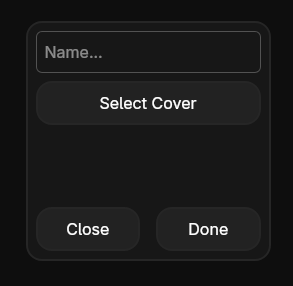
\includegraphics[width=0.6\textwidth]{media/screenshots/new_playlist.png}
                    \caption{Menú de nueva playlist}
                    \label{fig:nueva playlist}
                \end{figure}

                Cuando el atributo \verb|isModalOpen| de \verb|sidebar| cambia a \verb|true| se abre un menu modal donde es posible crear una nueva playlist vacía.

                Estos son los métodos más destacados:

                \begin{lstlisting}[caption={selectCover()}]
async selectCover() {
    const file = await open({
      multiple: false,
      directory: false,
    });

    if(file == null) {
      return
    }

    const fileData = await readFile(file);
    const ogBlob = new Blob([fileData], { type: 'image/*' });
    const thumbnail = await this.createThumbnail(ogBlob, 200, 200);

    try {
      await mkdir('pcovers', { baseDir: BaseDirectory.AppData });
    } catch {
      console.log("Already Created")
    }
    

    let randomName = (Math.floor(Math.random() * (Math.floor(200000) - Math.ceil(1) + 1)) + Math.ceil(1)).toString();
    await writeFile(`pcovers/${randomName}.jpg`, thumbnail, {baseDir: BaseDirectory.AppData})

    const data_dir = await appDataDir();
    let newPath = data_dir + "/pcovers/" + randomName + ".jpg";
    console.log(newPath)

    this.coverPath = newPath;
}
                \end{lstlisting}

                
                El método \verb|selectCover()| gestiona la selección y procesamiento de imágenes para las portadas de playlists mediante el siguiente flujo: cuando se pulsa sobre el botón \textit{Select Cover}, se activa un diálogo de selección de archivos utilizando el \verb|plugin-dialog| de Tauri. La imagen seleccionada se convierte en un objeto \verb|Blob| y se redimensiona mediante el método \verb|createThumbnail| para optimizar su almacenamiento. El archivo resultante se guarda en el directorio \verb|pcovers| dentro de la carpeta de datos de la aplicación, con un nombre generado aleatoriamente para evitar colisiones. Si el directorio no existe previamente, se crea automáticamente durante este proceso. La ruta final de la imagen procesada se asigna al atributo \verb|coverPath| para su uso en la interfaz.

                \begin{lstlisting}[caption={createThumbnail()}]
async createThumbnail(blob: Blob, maxWidth: number, maxHeight: number): Promise<Uint8Array> {
    return new Promise((resolve, reject) => {
        const img = new Image();
        img.onload = () => {
            const canvas = document.createElement('canvas');
            const scale = Math.min(
                maxWidth / img.width,
                maxHeight / img.height
            );
            canvas.width = img.width * scale;
            canvas.height = img.height * scale;
            
            const ctx = canvas.getContext('2d')!;
            ctx.drawImage(img, 0, 0, canvas.width, canvas.height);
            
            canvas.toBlob(async (thumbnailBlob) => {
                if (!thumbnailBlob) {
                    reject(new Error("Failed to create thumbnail blob"));
                    return;
                }
                
                try {
                    const arrayBuffer = await thumbnailBlob.arrayBuffer();
                    const uint8Array = new Uint8Array(arrayBuffer);
                    resolve(uint8Array);
                } catch (error) {
                    reject(error);
                }
            }, 'image/jpeg', 0.7);
        };
        
        img.onerror = () => {
            reject(new Error("Failed to load image"));
        };
        
        img.src = URL.createObjectURL(blob);
    });
}
                \end{lstlisting}

                El método \verb|createThumbnail()| implementa el proceso de redimensionamiento de imágenes mediante la Canvas API, siguiendo tres etapas principales: primero, se crea un objeto \verb|Image| y se carga el \verb|Blob| de entrada mediante \verb|URL.createObjectURL()|. Segundo, al completarse la carga, se calcula el factor de escala proporcional para mantener las dimensiones dentro de los límites especificados (\verb|maxWidth| y \verb|maxHeight|), creando un elemento \verb|canvas| con las nuevas dimensiones. Finalmente, se dibuja la imagen escalada en el canvas y se convierte a un \verb|Uint8Array| comprimido en formato JPEG con calidad del 70\%, manejando posibles errores durante el proceso mediante el sistema de promesas. Esta implementación garantiza un procesamiento eficiente de imágenes para su almacenamiento optimizado en el sistema de archivos. \\

                Una vez seleccionados la portada y el nombre de la playlist, al pulsar el boton \textit{done} se ejecuta el siguiente método, que realiza las siguientes acciones secuenciales:

                \begin{enumerate}
                    \item Envía una petición al backend implementado en Rust para crear la nueva playlist.
                    \item Cierra el menú modal de creación.
                    \item Actualiza la lista de playlist en la interfaz.
                    \item Restablece la imagen predeterminada en el atributo de la clase para futuras iteraciones (última línea del método).
                \end{enumerate}

                \begin{lstlisting}[caption={createPlaylist()}]
async createPlaylist() {
    const data_dir = await appDataDir();
    invoke('create_playlist', {name: this.name, cover_path: this.coverPath, db_path: data_dir})
    this.close()
    this.refresh()
    this.coverPath = "assets/black.jpg"
}
                \end{lstlisting}

                \paragraph{Boton Search}

                ‎ \\

                \begin{figure}[H]
                    \centering
                    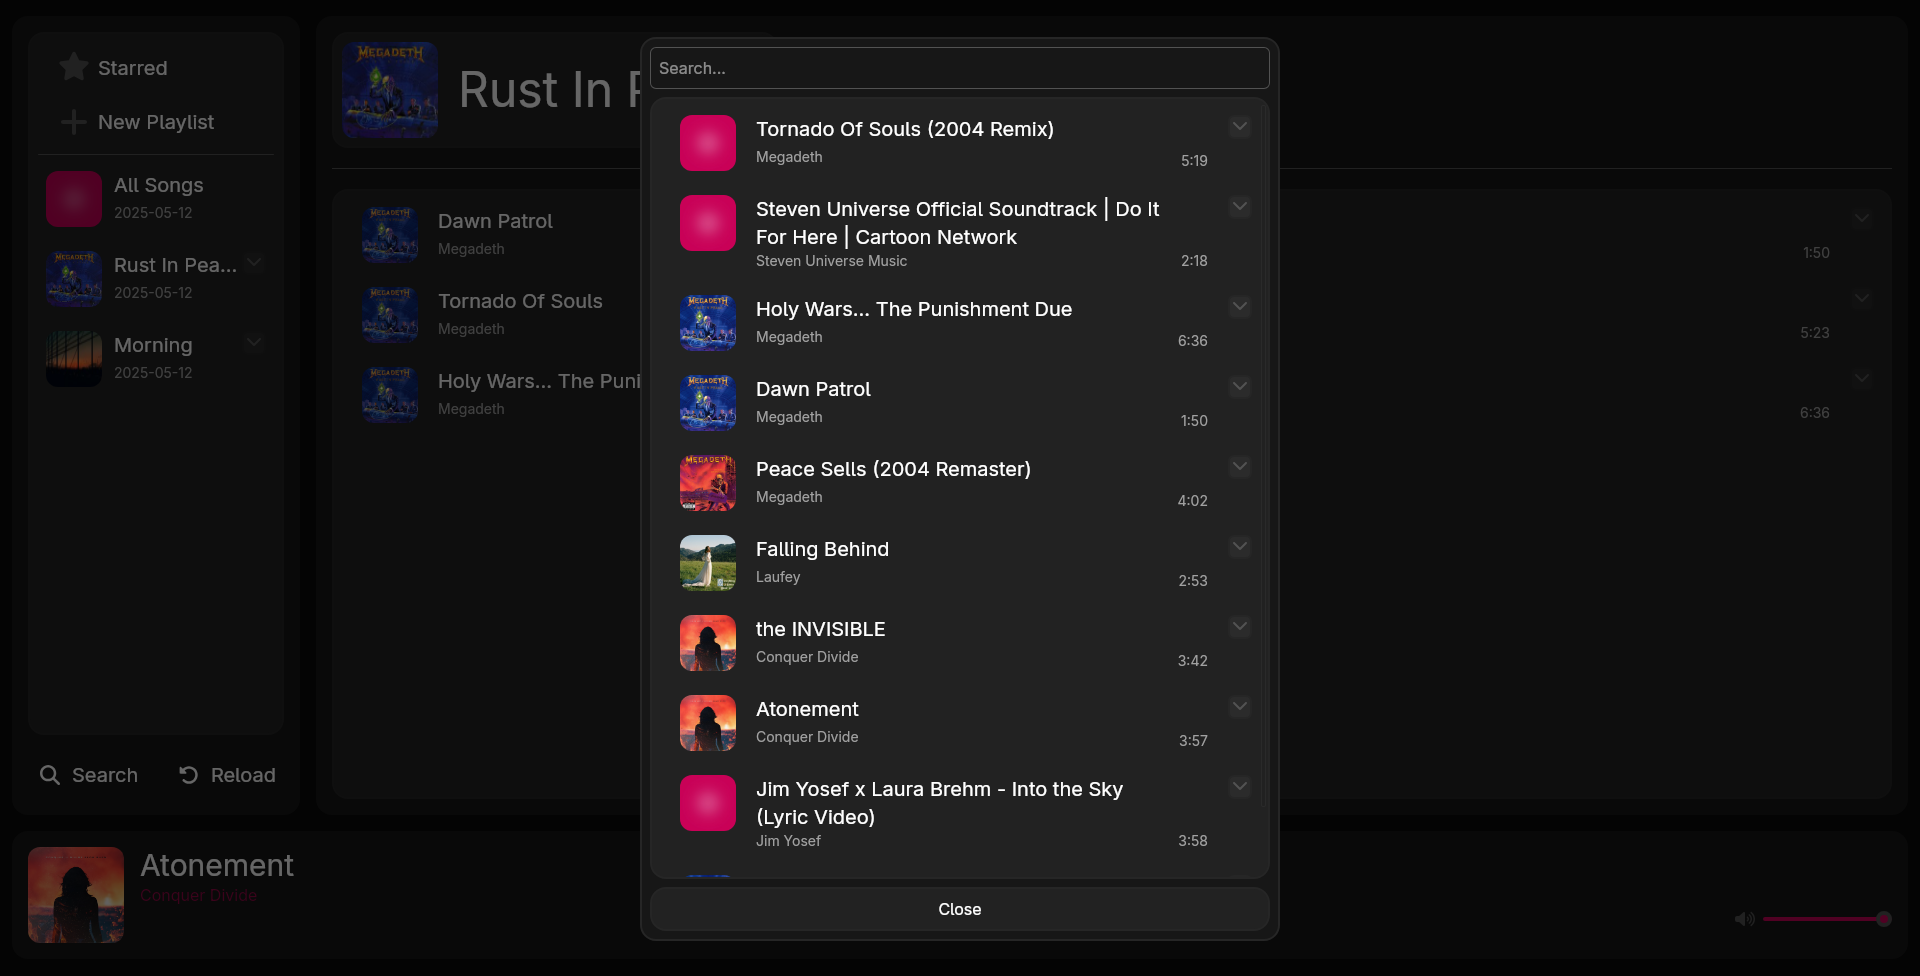
\includegraphics[width=0.8\textwidth]{media/screenshots/search_song.png}
                    \caption{Menú de buscar canción}
                    \label{fig:buscar}
                \end{figure}

                \begin{lstlisting}[caption={searchSong()}]
async searchSong() {
    await this.getAllSongs();
    this.filteredSongs = this.songs;
    this.isModalOpenSearch = true;
}

async getAllSongs() {
    const data_dir = await appDataDir();
    try {
      this.songs = await invoke<Song[]>('get_all_songs', {db_path: data_dir});
    } catch (error) {
      console.error('Error fetching songs:', error);
      this.songs = [];
    }
}
                \end{lstlisting}

                Cuando se activa la función de búsqueda mediante el botón correspondiente, se ejecuta el siguiente proceso: en primer lugar, se obtienen todas las canciones disponibles a través del método \verb|getAllSongs()|, que realiza una llamada al backend mediante Tauri IPC para recuperar los registros de la base de datos SQLite. Una vez completada esta operación, la lista completa de canciones se asigna a la variable \verb|filteredSongs| y se activa el modal de búsqueda estableciendo \verb|isModalOpenSearch| a \verb|true|. Este menú modal permite buscar y seleccionar canciones de toda la colección musical, ofreciendo las mismas capacidades de interacción que cuando las canciones se encuentran dentro de una playlist específica, funcionalidad que se detallará más adelante en la documentación.


            \subsubsection{Mainscreen}

            \begin{figure}[H]
                \centering
                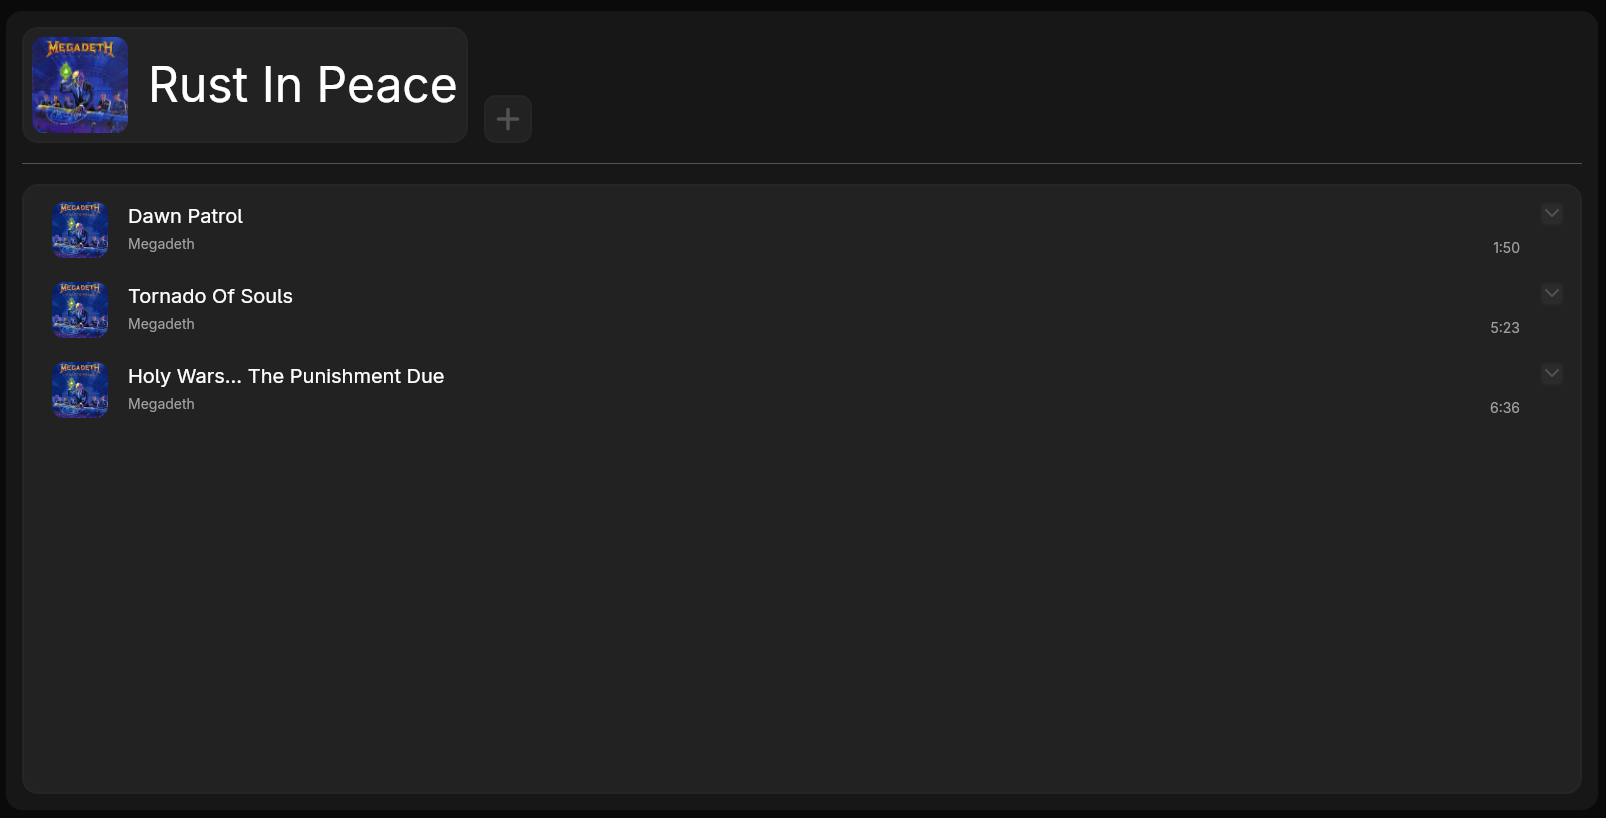
\includegraphics[width=1\textwidth]{media/screenshots/playlist.png}
                \caption{Mainscreen}
                \label{fig:Mainscreen}
            \end{figure}

            Este componente se encarga de mostrar la lista de canciones pertenecientes a una playlist, presentando para cada una:

            \begin{itemize}
                \item Información básica (título, artista, duración)
                \item Controles interactivos:
                \begin{itemize}
                    \item Botón de reproducción directa
                    \item Opción para añadir a la cola de reproducción
                \end{itemize}
            \end{itemize}

            La implementación de este componente sigue un principio de composición, donde la lógica sustancial se encuentra distribuida en sus subcomponentes especializados, mientras que el componente principal actúa principalmente como contenedor y coordinador de la visualización. \\

                \paragraph{Song Button}
                ‎

                \begin{figure}[H]
                    \centering
                    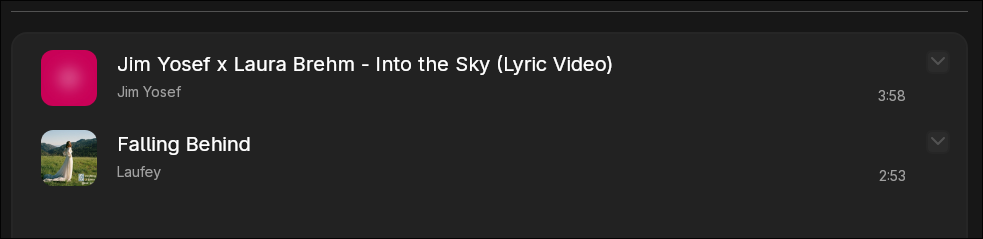
\includegraphics[width=1\textwidth]{media/screenshots/songbutton.png}
                    \caption{Song Button}
                    \label{fig:songbutton}
                \end{figure}

                Cada canción dentro de una playlist cuenta con un componente específico para su gestión y visualización de información. Al seleccionar el área principal del componente, se inicia automáticamente la reproducción del archivo de audio correspondiente. En la parte derecha del elemento se encuentra un menú desplegable (\textit{dropdown menu}) que proporciona las siguientes funcionalidades:

                \begin{itemize}
                    \item Añadir la canción a la cola de reproducción actual
                    \item Agregar la canción a otra playlist existente
                    \item Eliminar la canción de la playlist actual (función no disponible en la playlist \verb|All Songs|)
                \end{itemize}

                El concepto de \verb|All Songs|, que representa la colección completa de canciones disponibles, se explicará con mayor detalle en secciones posteriores de esta documentación.

                Los atributos del componente son:

                \begin{lstlisting}[caption={Atributos Song Button}]
isModalOpen: boolean = false;

isDropDownOpen: boolean = false;

constructor (public songManagement:SongManagementService, public songAdding:SongAddingService, public mainScreenStatus:MainScreenStatusService) {}

@Input() id!: string;
@Input() path!: string;
@Input() title!: string;
@Input() artist!: string;
@Input() album!: string;
@Input() year!: string;
@Input() duration!: string;
@Input() coverPath!: string;
@Input() isStarred!: boolean;

@Input() playlistId!: number;

coverUrl: string = 'assets/black.jpg';
                \end{lstlisting}

                Entre ellos se encuentran los metadatos de cada canción y la playlist en la que se encuentran mostrados ahora mismo. Estos datos son recibidos desde el componente padre. \\

                Además posee la interfaz \verb|Song|:

                \begin{lstlisting}[caption={Song}]
interface Song {
  id:string,
  path:string,
  title:string,
  artist:string,
  album:string,
  year:string,
  duration:string,
  coverPath:string,
  isStarred:boolean
}
                \end{lstlisting}

                El componente implementa diversos métodos para gestionar su funcionalidad, entre los cuales destaca:

                \begin{lstlisting}[caption={Dropdown menu}]
toggleDropDown() {
    this.isDropDownOpen = !this.isDropDownOpen;
}

closeDropDown() {
    this.isDropDownOpen = false;
}

@HostListener('document:click', ['$event'])
  onClickOutside(event: Event) {
    const target = event.target as HTMLElement;
    if (!target.closest('.relative.inline-block')) {
      this.closeDropDown();
    }
}
                \end{lstlisting}

                El menú desplegable (\textit{dropdown menu}) que contiene las opciones de gestión para cada canción implementa el siguiente comportamiento:

                \begin{itemize}
                    \item La visibilidad del menú se controla mediante el atributo booleano \verb|isDropDownOpen|
                    \item El método \verb|toggleDropDown()| alterna el estado de visibilidad
                    \item El método \verb|closeDropDown()| garantiza el cierre programático del menú
                \end{itemize}

                Para mejorar la experiencia de usuario, se implementa un cierre automático mediante el decorador \verb|@HostListener|, que detecta eventos de clic fuera del área del componente y ejecuta el cierre del menú cuando corresponde.

                \begin{lstlisting}[caption={playSong() y addSongToQueue()}]
playSong() {
    let song:Song = {id: this.id, path: this.path, title:this.title, artist: this.artist, album: this.album, year: this.year, duration: this.duration, coverPath: this.coverPath, isStarred: this.isStarred };
    this.songManagement.setOneSong(song);
}

addSongToQueue() {
    let song:Song = {id: this.id, path: this.path, title:this.title, artist: this.artist, album: this.album, year: this.year, duration: this.duration, coverPath: this.coverPath, isStarred: this.isStarred };
    this.songManagement.addOneSong(song);
}
                \end{lstlisting}

                Los métodos implementados siguen un patrón común donde los metadatos de la canción se estructuran en un objeto de tipo \verb|Song|, conteniendo todos los atributos relevantes (identificador, ruta, título, artista, álbum, año, duración, portada y estado de favorito). Este objeto se envía al servicio \verb|song-management|, diferenciándose en:

                \begin{itemize}
                    \item \verb|playSong()|: Inicia la reproducción inmediata mediante \verb|setOneSong()|
                    \item \verb|addSongToQueue()|: Añade la canción a la cola de reproducción usando \verb|addOneSong()|
                \end{itemize}

                \begin{lstlisting}[caption={addSongToPlaylist()}]
addSongToPlaylist() {
    this.songAdding.getAllPlaylists();
    this.isModalOpen = true;
}

close() {
    this.isModalOpen = false;
    this.songAdding.letGo();
}
                \end{lstlisting}

                El flujo de añadir canciones a playlists sigue un proceso estructurado:

                \begin{itemize}
                    \item \textbf{Fase de preparación}:
                    \begin{itemize}
                        \item Se obtienen todas las playlists disponibles mediante el servicio \verb|song-adding|.
                        \item Se activa el modal de selección estableciendo \verb|isModalOpen| a \verb|true|.
                    \end{itemize}
                    
                    \item \textbf{Fase de cierre}:
                    \begin{itemize}
                        \item Al completar la operación, se desactiva el modal (\verb|isModalOpen = false|).
                        \item Se liberan los recursos del servicio mediante \verb|letGo()| para optimizar memoria.
                    \end{itemize}
                \end{itemize}

                Este diseño garantiza una gestión eficiente de recursos durante el proceso de agregado de canciones a playlists.

                \begin{lstlisting}[caption={removeSongFromPlaylist()}]
async removeSongFromPlaylist() {
    const data_dir = await appDataDir();
    invoke('remove_song_from_playlist', {playlist_id: this.playlistId, song_id: this.id, db_path: data_dir});
    this.mainScreenStatus.refresh();
}
                \end{lstlisting}

                Cuando se activa la eliminación de una canción mediante el botón correspondiente, se ejecuta una petición al backend implementado en Rust que procesa la eliminación del registro en la base de datos SQLite. El método obtiene primero la ruta del directorio de datos mediante \verb|appDataDir()|, luego envía los parámetros necesarios (identificador de playlist, identificador de canción y ruta de la base de datos) a través de la función \verb|invoke()|. Finalmente, se actualiza el estado de la interfaz principal llamando al método \verb|refresh()| del servicio \verb|mainScreenStatus|, lo que garantiza que los cambios se reflejen inmediatamente en la vista del usuario.

                \begin{lstlisting}[caption={toggleStarred()}]
async toggleStarred() {
    const data_dir = await appDataDir();
    
    if (this.isStarred) {
      invoke('remove_is_starred', {song_id: this.id, db_path: data_dir});
      console.log("Canción !Starred: " + this.id);
    } else {
      invoke('add_is_starred', {song_id: this.id, db_path: data_dir});
      console.log("Canción Starred: " + this.id);
    }

    this.mainScreenStatus.refresh();
}
                \end{lstlisting}

                El método \verb|toggleStarred()| gestiona el estado de favorito de las canciones mediante un proceso que alterna entre dos posibles acciones. Cuando una canción está marcada como favorita (\verb|isStarred = true|), se ejecuta la función \verb|remove_is_starred| en el backend de Rust para eliminarla de la lista especial. En caso contrario, se invoca \verb|add_is_starred| para añadirla. En ambos casos, se utiliza \verb|appDataDir()| para obtener la ruta de la base de datos y se actualiza la interfaz mediante \\ \verb|mainScreenStatus.refresh()|. Las canciones marcadas como favoritas se agrupan automáticamente en una playlist especial accesible desde un botón específico en la barra lateral de la aplicación.

                \paragraph{Playlist Button}
                ‎

                Este componente de interfaz se activa exclusivamente cuando se inicia el menú modal para añadir canciones a playlists.

                Estos son sus atributos:

                \begin{lstlisting}[caption={Atributos Playlist Button}]
coverPath = 'assets/black.jpg';

constructor (public mainScreenStatus:MainScreenStatusService) {}

@Input() playlistId!: number;

@Input() playlistName!: string;

@Input() playlistCoverPath!: string;

@Input() songId!: string;
                \end{lstlisting}

                Su funcionamiento principal consiste en presentar al usuario la lista completa de playlists disponibles en el sistema, permitiendo la selección del destino donde se agregará la canción actual. \\

                Sus métodos más importantes son:

                \begin{lstlisting}[caption={getCoverPath()}]
async ngOnInit() {
    this.coverPath = await this.getCoverPath();
}

async getCoverPath(): Promise<string> {
    if (!this.coverPath) return 'assets/black.jpg';

    const fileData = await readFile(this.playlistCoverPath);

    const blob = new Blob([fileData], { type: 'image/jpeg' });

    if (this.coverPath) {
        URL.revokeObjectURL(this.coverPath);
    }

    return URL.createObjectURL(blob);
}
                \end{lstlisting}

                Este método, que sigue la misma implementación ya descrita en el componente anterior, se encarga de gestionar la visualización de las portadas de las playlists.

                \begin{lstlisting}[caption={addSongToPlaylist()}]
async addSongToPlaylist() {
    const data_dir = await appDataDir();
    invoke('add_song_to_playlist', {playlist_id: this.playlistId, song_id: this.songId, db_path: data_dir})
    this.mainScreenStatus.refresh();
}
                \end{lstlisting}

                El método \verb|addSongToPlaylist()| ejecuta el proceso de añadir una canción a una playlist específica mediante una llamada al backend implementado en Rust. Primero obtiene el directorio de datos de la aplicación usando \verb|appDataDir()|, luego envía los parámetros necesarios (ID de la playlist, ID de la canción y ruta de la base de datos) a través de la función \verb|invoke()|. Finalmente, actualiza la página principal llamando a \verb|mainScreenStatus.refresh()| para reflejar los cambios en la interfaz de usuario. Este flujo garantiza que la canción quede registrada en la base de datos y que la vista se actualice consistentemente.

                \paragraph{Homeitem}
                ‎

                El componente \verb|Homeitem| representa una implementación alternativa al componente estándar \verb|Song|, desarrollado específicamente para cumplir con requerimientos particulares de diseño y funcionalidad en la playlist \textit{Starred Songs}.

            \subsubsection{Servicios}

            Se han implementado servicios especializados para cada funcionalidad clave, tales como el manejo de listas de reproducción, la gestión de metadatos musicales y la información de la \verb|mainscreen|.

                \paragraph{Main Screen Status}
                ‎

                \begin{lstlisting}[caption={Atributos Main Screen Status}]
onHome = signal(true);
pId: number = 0;
pName: string = "";
pDate: string = "";
pCoverPath: string = "";
pStarred: boolean = false;

songs:Song[] = []

constructor(public songManagement:SongManagementService) { }
                \end{lstlisting}

                El servicio \verb|MainScreenStatus| se encarga de gestionar y mantener el estado de la información mostrada en la interfaz principal de la aplicación (\verb|mainscreen|). Para ello, se han definido una serie de atributos que almacenan tanto los metadatos de la playlist actualmente visualizada como las canciones asociadas a la misma.

                Entre los atributos principales se incluyen señales y variables que controlan el estado de la interfaz (\verb|onHome|), así como información específica de la playlist, como su identificador (\verb|pId|), nombre (\verb|pName|), fecha de creación (\verb|pDate|), ruta de la portada (\verb|pCoverPath|) y estado de favorito (\verb|pStarred|). Adicionalmente, se almacena un arreglo de canciones (\verb|songs|) que pertenecen a la playlist actual. Por supuesto este servicio contiene la interfaz \verb|Song| vista anteriormente.

                El servicio se inicializa con una dependencia inyectada del \\ \verb|SongManagementService|, lo que permite una coordinación fluida entre la gestión del estado de la interfaz y las operaciones relacionadas con la reproducción de audio. Esta arquitectura modular facilita el mantenimiento y la escalabilidad del código. \\


                \begin{lstlisting}[caption={setHome() y setPlaylist()}]
setHome() {
    this.onHome.set(true);
    this.pId = 0;
    this.pName = "";
    this.pDate = "";
    this.pCoverPath = "";
    this.getAllStarred();
}

setPlaylist(id:number, name:string, date:string, coverPath:string, isStarred:boolean) {
    this.onHome.set(false);
    this.pId = id;
    this.pName = name;
    this.pDate = date;
    this.pCoverPath = coverPath;
    this.pStarred = isStarred;
}
                \end{lstlisting}

                Los métodos \verb|setHome()| y \verb|setPlaylist()| gestionan la transición entre las diferentes vistas de la interfaz principal (\verb|mainscreen|). En el primer caso, \verb|setHome()| configura el estado para mostrar la lista de canciones marcadas como favoritas, estableciendo el valor \verb|onHome| a \verb|true| y reiniciando los metadatos de la playlist. Simultáneamente, se invoca el método \verb|getAllStarred()| para cargar las canciones destacadas.

                Por otro lado, \verb|setPlaylist()| se utiliza para visualizar una playlist específica, actualizando los metadatos correspondientes (\verb|id|, \verb|name|, \verb|date|, \verb|coverPath| y estado \verb|isStarred|) y desactivando la vista de favoritos mediante \verb|onHome.set(false)|.

                Cabe destacar que la nomenclatura original (\verb|Home|) fue heredada de las primeras etapas del desarrollo, cuando la estructura conceptual del proyecto aún estaba en definición. Posteriormente, esta terminología se actualizó a \verb|Starred Songs| para reflejar con mayor precisión su funcionalidad. A pesar de este cambio, se mantuvieron las referencias originales en el código para preservar la compatibilidad con los componentes existentes.

                Se ha considerado una refactorización futura para unificar la nomenclatura y mejorar la coherencia del código. Actualmente, aunque los términos \verb|Home| y \verb|Starred Songs| coexisten, esta dualidad no afecta la funcionalidad del sistema. \\

                \begin{lstlisting}[caption={Obtención de playlists}]
async getAllSongs() {
    const data_dir = await appDataDir();
    try {
      this.songs = await invoke<Song[]>('get_all_songs', {db_path: data_dir});
    } catch (error) {
      console.error('Error fetching songs:', error);
      this.songs = [];
    }
}

async getAllStarred() {
    const data_dir = await appDataDir();
    try {
      this.songs = await invoke<Song[]>('get_all_starred', {db_path: data_dir});
    } catch (error) {
      console.error('Error fetching songs:', error);
      this.songs = [];
    }
}

async getPlaylistSongs() {
    const data_dir = await appDataDir();
    try {
      this.songs = await invoke<Song[]>('get_playlist_songs', {playlist_id: this.pId, db_path: data_dir});
    } catch (error) {
      console.error('Error fetching songs:', error);
      this.songs = [];
    }
}
                \end{lstlisting}

                Los métodos \verb|getAllSongs()|, \verb|getAllStarred()| y \verb|getPlaylistSongs()| gestionan la obtención de canciones desde diferentes fuentes, asignándolas posteriormente a la variable local \verb|songs|. En cada caso, se sigue un patrón similar: primero se obtiene el directorio de datos de la aplicación mediante \verb|appDataDir()|, luego se realiza una llamada al backend mediante \verb|invoke()|, y finalmente se manejan tanto el éxito como los posibles errores de la operación.

                \begin{lstlisting}[caption={refresh()}]
async refresh() {
    if (this.pId != 0) {
      await this.getPlaylistSongs();
    } else if (this.pId == 0 && this.onHome()) {
      await this.getAllStarred();
    } else {
      await this.getAllSongs();
    }
}
                \end{lstlisting}

                El método \verb|refresh()| se encarga de actualizar dinámicamente el contenido mostrado en la \verb|mainscreen| en función del contexto actual de reproducción. Para ello, se implementa un flujo condicional que evalúa el identificador de playlist almacenado en \verb|this.pId| y el estado de la señal \verb|onHome|.

                Este enfoque garantiza que la interfaz siempre muestre el contenido más relevante según el estado actual de la aplicación, manteniendo una experiencia de usuario coherente. La implementación mediante llamadas asíncronas (\verb|await|) asegura que las operaciones de actualización se completen antes de proceder con cualquier otra acción, evitando así condiciones de carrera o estados inconsistentes en la interfaz.

                \begin{lstlisting}[caption={playQueue() y addQueue()}]
playQueue() {
    this.songManagement.setQueue(this.songs);
  }

addQueue() {
    this.songManagement.addQueue(this.songs);
}
                \end{lstlisting}

                Estos métodos gestionan la interacción con la cola de reproducción a través del servicio \verb|SongManagementService|. Al pulsar sobre el nombre de la playlist, se invoca \verb|playQueue()|, que establece la lista actual de canciones (\verb|this.songs|) como nueva cola de reproducción mediante el método \verb|setQueue()| del servicio. De forma similar, al seleccionar la opción de añadir a cola, \verb|addQueue()| incorpora las canciones a la cola existente utilizando \verb|addQueue()| del mismo servicio.

                Esta implementación refleja una arquitectura limpia donde la lógica de gestión de reproducción se delega completamente al servicio, permitiendo que los componentes se centren únicamente en la presentación de datos y captura de eventos de usuario. El servicio \\ \verb|SongManagementService| será analizado en profundidad en la siguiente sección de esta documentación.

                \paragraph{Song Management}
                ‎

                \begin{lstlisting}[caption={Atributos Song Management}]
songCover:string = ""
songTitle:string = ""
songArtist:string = ""

constructor() { this.setupSongListeners() }

song: HTMLAudioElement = new Audio();

volume:number = 0;

isPlaying:boolean = false;

loopMode:string = "none" //* none - playlist - single
shuffle:boolean = false

queue:Song[] = []
queueSave:Song[] = []
currentIndex:number = 0
currentIndexSave:number = 0
currentISDelay:number = 0

progress:number = 0;
                \end{lstlisting}

                El servicio \verb|SongManagementService| centraliza toda la lógica relacionada con la reproducción musical y gestión de colas en la aplicación. Sus atributos principales pueden categorizarse en tres grupos:

                \begin{enumerate}
                    \item \textbf{Metadatos visuales}: Almacena información de la canción actual (\verb|songCover|, \verb|songTitle|, \verb|songArtist|) para mostrarse en la interfaz.
                    \item \textbf{Control de reproducción}: Incluye el elemento \verb|HTMLAudioElement| para manejo nativo del audio, junto con estados como \verb|isPlaying|, \verb|volume| y \verb|progress| que reflejan la reproducción en tiempo real.
                    \item \textbf{Gestión de cola}: Mantiene dos versiones de la cola (\verb|queue| y \verb|queueSave|) para implementar funcionalidades como shuffle, junto con índices de posición (\verb|currentIndex|, \verb|currentIndexSave|) y modos especiales (\verb|loopMode|, \verb|shuffle|).
                \end{enumerate}

                El constructor inicializa automáticamente los listeners de eventos mediante \verb|setupSongListeners()|, preparando el servicio para responder a cambios de estado.

                \begin{lstlisting}[caption={setUpSongListeners()}]
private async setupSongListeners() {
    this.song?.addEventListener('ended', () => this.playNext());
    this.song?.addEventListener('timeupdate', () => {
      if (this.song) {
        this.progress = (this.song.currentTime / this.song.duration) * 100;
      }
    });
}
                \end{lstlisting}

                El método \verb|setupSongListeners()| configura los listeners esenciales para el control de reproducción, implementando dos funcionalidades clave mediante eventos sobre el elemento \verb|HTMLAudioElement|.
                
                \begin{enumerate}
                    \item El evento 'ended' activa automáticamente \verb|playNext()| al terminar la canción actual, permitiendo una reproducción continua.
                    \item Segundo, el evento 'timeupdate' actualiza constantemente la propiedad \verb|progress| con el porcentaje de avance (calculado como la relación entre \verb|currentTime| y \verb|duration|), lo que se refleja en la barra de progreso de la interfaz.
                \end{enumerate}

                \begin{lstlisting}[caption={getCoverPath()}]
async getCoverPath(coverPath:string): Promise<string> {
    let coverUrl: string = 'assets/black.jpg';
    if (!coverPath) return coverUrl;

    const fileData = await readFile(coverPath);
    
    const blob = new Blob([fileData], { type: 'image/jpeg' });

    if (coverUrl) {
      URL.revokeObjectURL(coverUrl);
    }

    return URL.createObjectURL(blob);

}
                \end{lstlisting}

                El método \verb|getCoverPath()| representa una solución centralizada para la gestión de portadas de las canciones, cuya implementación fue migrada desde el componente \verb|playbar| al servicio actual como parte de una refactorización para simplificar la arquitectura. Esta implementación unificada elimina la duplicación de código que existía cuando la funcionalidad estaba dispersa en varios componentes (a excepción de las playlists), mejorando el mantenimiento y permitiendo una gestión más eficiente de los recursos multimedia.

                \begin{lstlisting}[caption={loadAndPlay()}]
async loadAndPlay(_path:string, _index:number) {
    try {
      this.songTitle = this.queue[_index].title;
      this.songArtist = this.queue[_index].artist;
      
      this.songCover = await this.getCoverPath(this.queue[_index].coverPath);

      const path = _path;
      
      const fileData = await readFile(path);
      const blob = new Blob([fileData], { type: 'audio/mp3' });
      const audioUrl = URL.createObjectURL(blob);
      
      this.song.src = audioUrl;
      await this.song.play();
      this.isPlaying = true;
      
      console.log('Canción cargada correctamente');
    } catch (error) {
      console.error('Error al cargar la canción:', error);
    }
}
                \end{lstlisting}

                El método \verb|loadAndPlay()| gestiona todo el proceso de preparación y reproducción de canciones mediante un flujo secuencial. Primero actualiza los metadatos visuales (\verb|songTitle|, \verb|songArtist| y \verb|songCover|) utilizando los datos de la canción en la posición \verb|_index| de la cola. Para la portada, se emplea el método \verb|getCoverPath()| previamente descrito. Luego carga el archivo de audio desde la ruta especificada (\verb|_path|), lo convierte a un blob y genera una URL temporal para su reproducción. Finalmente asigna esta URL al elemento de audio (\verb|this.song.src|) e inicia la reproducción, actualizando el estado \verb|isPlaying|. Todo el proceso está encapsulado en un bloque try-catch que maneja posibles errores durante la carga.

                \begin{lstlisting}[caption={set y add}]
setQueue(songs:Song[]) {
    this.queue = [...songs];
    this.currentIndex = 0;
    this.loadAndPlay(this.queue[0].path, 0);
}

addQueue(songs: Song[]) {
    this.queue.push(...songs)
}

setOneSong(song:Song) {
    this.queue = [];
    this.queue.push(song);
    this.currentIndex = 0;
    this.loadAndPlay(this.queue[0].path, 0);
}

addOneSong(song:Song) {
    this.queue.push(song);
}
                \end{lstlisting}

                Estos métodos constituyen la API fundamental para la gestión de la cola de reproducción, mencionada recurrentemente en secciones anteriores de la documentación. La implementación sigue un patrón dual con variantes "set" (establecer) y "add" (añadir):

                Los métodos \verb|setQueue()| y \verb|setOneSong()| reemplazan completamente la cola existente. En el primer caso, se recibe un array de canciones que se copia mediante el operador de propagación (\verb|...songs|), mientras que el segundo acepta una única canción, reiniciando la cola antes de añadirla. Ambos métodos comparten el mismo flujo posterior: reinician el índice actual a 0 e invocan \verb|loadAndPlay()| para comenzar la reproducción inmediata.

                Por otro lado, \verb|addQueue()| y \verb|addOneSong()| implementan la funcionalidad complementaria de añadir contenido a la cola existente sin modificar el estado de reproducción actual. La versión \verb|addQueue()| utiliza el mismo operador de propagación para incorporar múltiples canciones, mientras que \verb|addOneSong()| trabaja con elementos individuales.

                \begin{lstlisting}[caption={togglePlayPause()}]
async togglePlayPause() {
    if(!this.isPlaying) {
      this.song.play()
    } else {
      this.song.pause()
    }
    this.isPlaying = !this.isPlaying;
}
                \end{lstlisting}
                 
                El método \verb|togglePlayPause()| implementa la funcionalidad básica de control de reproducción mediante un mecanismo de alternancia. Cuando se invoca, verifica el estado actual de reproducción a través de la variable \verb|isPlaying|. Si la reproducción está pausada (\verb|isPlaying| es falso), se ejecuta el método \verb|play()| del elemento de audio HTML. En caso contrario, se activa el método \verb|pause()|. Finalmente, se invierte el valor de \verb|isPlaying| para reflejar el nuevo estado.

                \begin{lstlisting}[caption={playNext() y playPrevious()}]
playNext() {
    if ((this.currentIndex < this.queue.length - 1) && (this.loopMode == "none" || this.loopMode == "playlist")) {
      this.currentIndex++;
      this.currentISDelay++;
      this.loadAndPlay(this.queue[this.currentIndex].path, this.currentIndex);
    } else if ((this.currentIndex == this.queue.length - 1) && this.loopMode == "playlist") {
      this.currentIndex = 0;
      this.loadAndPlay(this.queue[this.currentIndex].path, this.currentIndex);
    } else if (this.loopMode == "single") {
      this.song.currentTime = 0
    } else {
      this.stop();
    }
    console.log("CurrentIndex: " + this.currentIndex + " CurrentIndexSave: " + this.currentIndexSave)
}

playPrevious() {
    if(this.song.currentTime < 3) {
      if((this.currentIndex > 0) && this.loopMode != "single") {
        this.currentIndex--;
        this.currentISDelay--;
        this.loadAndPlay(this.queue[this.currentIndex].path, this.currentIndex);
      } else if (this.currentIndex == 0) {
        if (this.loopMode == "playlist") {
          this.currentIndex = this.queue.length - 1
          this.loadAndPlay(this.queue[this.currentIndex].path, this.currentIndex);
        } else if(this.loopMode == "single") {
          this.song.currentTime = 0
        } else {
          this.stop()
        }
      } else {
        this.song.currentTime = 0
      }
    } else {
      this.song.currentTime = 0
    }
    
}

stop() {
    this.song.pause();
    this.song.currentTime = 0;
    this.isPlaying = false;
}
                \end{lstlisting}

                Estos métodos implementan la lógica avanzada de navegación en la cola de reproducción, considerando diferentes modos de funcionamiento (\verb|none|, \verb|playlist| y \verb|single|). En \verb|playNext()|, se evalúa primero si hay canciones siguientes disponibles y el modo de repetición lo permite, incrementando entonces el índice y cargando la siguiente canción. Cuando se alcanza el final de la lista en modo \verb|playlist|, se reinicia al principio. Para el modo \verb|single|, simplemente se reinicia la canción actual.

                El método \verb|playPrevious()| incorpora lógica adicional para diferenciar entre retroceder a la canción anterior (si la reproducción actual lleva menos de 3 segundos) o reiniciar la canción actual. Maneja correctamente los casos especiales como el inicio de la lista en modo \verb|playlist| (saltando al final) o el comportamiento específico del modo \verb|single|. Ambos métodos mantienen actualizados los índices de posición (\verb|currentIndex|, \verb|currentISDelay|) y registran el estado actual para depuración.

                La implementación demuestra un manejo robusto de todos los casos posibles de navegación, proporcionando una experiencia de usuario consistente con los reproductores musicales profesionales. El diseño modular permite fácil extensión para añadir nuevos modos de reproducción o comportamientos especiales en futuras iteraciones.

                \begin{lstlisting}[caption={Control de tiempo y volumen}]
onInput(event: Event) {
    const input = event.target as HTMLInputElement;
    const newTime = parseInt(input.value);
    if (this.song) {
      this.song.currentTime = newTime;
    }
}

onVolume(event: Event) {
    const inputVolume = event.target as HTMLInputElement;
    const newVolume = parseInt(inputVolume.value) / 100;
    if (this.song) {
      this.song.volume = newVolume;
    }
    this.volume = parseInt(inputVolume.value);
    return this.volume
}
                \end{lstlisting}

                Estos métodos gestionan la interacción del usuario con los controles de reproducción. El método \verb|onInput()| se encarga de actualizar la posición de reproducción cuando el usuario manipula la barra de progreso. Primero obtiene el valor del elemento HTML que generó el evento, lo convierte a número entero y luego actualiza la propiedad \verb|currentTime| del elemento de audio si este está disponible.

                Por su parte, \verb|onVolume()| controla los ajustes de volumen mediante un flujo similar: captura el valor del control deslizante de volumen, lo normaliza dividiendo entre 100 (para adaptarlo al rango 0-1 que espera el API de audio) y aplica este valor tanto al elemento de audio como a la variable local \verb|volume|. La conversión de tipos y normalización de valores garantiza que los controles funcionen consistentemente aunque provengan de diferentes fuentes de entrada.

                Ambos métodos implementan una verificación de existencia (\verb|if (this.song)|) como medida de seguridad para evitar errores cuando no hay elemento de audio inicializado.

                \begin{lstlisting}[caption={cycleLoop()}]
cycleLoop() {
    switch (this.loopMode) {
      case "none":
        this.loopMode = "playlist";
        break;
      case "playlist":
        this.loopMode = "single";
        break;
      case "single":
        this.loopMode = "none";
        break;
      default:
        this.loopMode = "none";
        break;
    }
    return this.loopMode;
}
                \end{lstlisting}

                Este método se encarga de alternar cíclicamente la variable \verb|loopMode|.

                \begin{lstlisting}[caption={Shuffle}]
toggleShuffle() {
    if(!this.shuffle) {
      this.queueSave = [...this.queue];
      this.currentIndexSave = this.currentIndex;
      this.doShuffle();
    } else if(this.shuffle) {
      this.currentIndex = this.queueSave.indexOf(this.queue[this.currentIndex]);
      this.queue = this.queueSave;
    }
    this.shuffle = !this.shuffle;
    return this.shuffle;
  }

doShuffle() {
    this.queue.unshift(this.queue[this.currentIndex])
    this.queue.splice(this.currentIndex+1,1)
    this.currentIndex = 0
    let firstElement = this.queue[0]
    let queueToShuffle = this.queue.splice(1);
    let currentIndex2 = queueToShuffle.length;

    while (currentIndex2 != 0) {

      let randomIndex = Math.floor(Math.random() * currentIndex2);
      currentIndex2--;

      [queueToShuffle[currentIndex2], queueToShuffle[randomIndex]] = [queueToShuffle[randomIndex], queueToShuffle[currentIndex2]];
    }
    queueToShuffle.unshift(firstElement)
    this.queue = queueToShuffle
    
}
                \end{lstlisting}

                La implementación del modo aleatorio (\textit{shuffle}) sigue un enfoque de dos fases mediante los métodos \verb|toggleShuffle()| y \verb|doShuffle()|. Cuando se activa el modo aleatorio, \verb|toggleShuffle()| preserva el estado original de la cola (\verb|queueSave|) y la posición actual (\verb|currentIndexSave|) antes de aplicar la aleatorización. Este diseño permite restaurar el orden inicial cuando se desactiva la función, manteniendo la coherencia con el comportamiento de reproductores profesionales.

                El método \verb|doShuffle()| implementa el algoritmo Fisher-Yates para la mezcla aleatoria, optimizado para garantizar que la canción actual permanezca en primera posición durante la transición. El proceso consta de tres etapas: (1) extracción y protección de la canción en reproducción, (2) mezcla aleatoria del resto de la cola mediante intercambios indexados, y (3) reconstrucción de la cola con la canción actual preservada. Esta implementación demuestra especial atención al detalle en la experiencia de usuario, evitando saltos bruscos en la reproducción durante la activación del modo aleatorio.

                El sistema mantiene sincronizados los estados paralelos (colas original y aleatoria, índices de posición) mediante operaciones atómicas, garantizando consistencia incluso en listas extensas. La solución combina eficiencia computacional (complejidad O(n) para la mezcla) con un diseño intuitivo que refleja los patrones de uso establecidos en aplicaciones de referencia del sector.

        \subsection{Backend}

        Rust y SQLite

            \subsubsection{Tauri API}

            \subsubsection{Sync method}

            \subsubsection{SQL CRUD}


\section{Conclusiones}

        \subsection{Logros principales}

        Se ha desarrollado con éxito un reproductor de música multiplataforma (Linux, MacOs y Windows) utilizando Tauri, que cumple con los objetivos principales de:

        \begin{itemize}
            \item Optimización de recursos (Mucho menor consumo de ram respecto a otras webapps basadas en Electro).
            \item Compatibilidad de formatos de audio (FLAC, MP3, etc...).
            \item Arquitectura modular para el desarrollo futuro.
        \end{itemize}

        \subsection{Dificultades clave}

        El principal desafío técnico fue la curva de aprendizaje asociada a Rust, lenguaje de programación de sistemas con el que no se contaba experiencia previa. Esta dificultad se resolvió mediante el estudio de documentación oficial, tutoriales especializados y la implementación de pruebas piloto. Adicionalmente, fue necesario adaptar los conocimientos existentes en desarrollo web al framework Angular, cuyo paradigma de componentes requirió un período de adaptación.

        \subsection{Valoración global}

        A pesar de las dificultades, el proyecto valida el potencial de Tauri para aplicaciones de audio eficientes, ofreciendo un rendimiento superior al de frameworks tradicionales. La escalabilidad de la arquitectura permite añadir funcionalidades como cambios en la apariencia en futuras iteraciones.

\printbibliography
\end{document}